\documentclass[preview]{standalone}

\usepackage{amsmath}
\usepackage{amssymb}
\usepackage{stellar}
\usepackage{definitions}
\usepackage{bettelini}
\usepackage{tikz}
\usepackage{pgfplots}

\begin{document}

\id{geoeconomica-telecomunicazioni}
\genpage

\section{Le telecomunicazioni}

\subsection{Digital divide}

\begin{snippetdefinition}{digital-divide-definition}{Digital divide}
    Il \textit{digital divide} è il divario presente tra chi ha accesso
    (adeguato) a internet e chi non lo possiede (per
    scelta o meno).
\end{snippetdefinition}

\begin{snippet}{digital-divide-items}
    \vspace{-1cm}
    \begin{itemize}
        \item Il digital divide è il divario nell'accesso a internet tra chi ha e chi non ha
            accesso adeguato;
        \item Questo divario causa l'esclusione dai benefici della società digitale, con
            conseguenze socio-economiche e culturali negative;
        \item Le forme di Digital Divide includono:
            \begin{itemize}
                \item Divario intergenerazionale, che colpisce principalmente gli anziani;
                \item Divario di genere, che colpisce donne non occupate o in condizioni particolari;
                \item Divario linguistico-culturale, che colpisci gli immigrati;
                \item Divario legato alla disabilità;
                \item Divario di scolarizzazione, che colpisce persone con bassi livelli di istruzione;
            \end{itemize}
        \item È una nuova forma di disuguaglianza sociale emersa dalla metà degli anni '90;
        \item Gli approcci per descrivere l'evoluzione di questo fenomeno sono:
            \begin{itemize}
                \item Approccio della normalizzazione, che prevede l'eliminazione progressiva del
                    divario;
                \item Approccio della stratificazione, che prevede un incremento delle
                    disuguaglianze digitali;
            \end{itemize}
        \item I tipi di divario sociale legati al fenomeno sono:
            \begin{itemize}
                \item Divario globale, che si riferisce alle differenze tra paesi sviluppati e
                    non sviluppati;
                \item Divario sociale, che riguarda le disuguaglianze all'interno di un singolo
                    paese;
                \item Divario democratico, che si riferisce alla partecipazione politica e sociale
                    influenzata dall'uso delle tecnologie.
            \end{itemize}
    \end{itemize}
\end{snippet}

\subsection{Flussi finanziari}

\begin{snippet}{flussi-finanziari-items}
    \vspace{-1cm}
    \begin{itemize}
        \item Le borse sono luoghi di scambio di azioni, prodotti finanziari, obbligazioni e valute;
        \item Lo sviluppo delle telecomunicazioni facilita scambi finanziari globali in tempo reale;
        \item Le borse più importanti si trovano a New York, Tokyo, Londra, Shanghai e Hong Kong;
        \item Le conseguenze negative della globalizzazione finanziaria includono:
            \begin{itemize}
                \item La deregolamentazione, che ha aumentato il numero di operatori non
                    trasparenti;
                \item L'uso di paradisi fiscali, che favorisce la criminalità organizzata, il
                    terrorismo e attività legali;
            \end{itemize}
        \item La dematerializzazione finanziaria ha portato a:
            \begin{itemize}
                \item Innovazione digitale che intensifica gli ordini di acquisto e vendita in
                    tempo reale;
                \item Trasferimento rapido di capitale tra settori e pacchetti azionari;
                \item Investimenti in prodotti finanziari che scambiano denaro presente con denaro
                    futuro;
            \end{itemize}
        \item Esempi di dematerializzazione includono:
            \begin{itemize}
                \item Negoziazioni ad alta frequenza che permettono movimenti di capitale rapidi;
                \item Crisi finanziarie internazionali, come la svalutazione della moneta
                    thailandese nel 1997.
            \end{itemize}
    \end{itemize}
\end{snippet}

\begin{snippet}{adozione-tecnologia-svizzera-illustration}
    \begin{center}
    \begin{figure*}[ht!]
        \definecolor{darkgreen}{rgb}{0.0, 0.5, 0.0}
        \centering
        \begin{tikzpicture}
        \begin{axis}[
            width=\textwidth,
            height=0.6\textwidth,
            xlabel={Anno},
            ylabel={Abbonamenti per 100 persone},
            xmin=1960, xmax=2022,
            ymin=0, ymax=140,
            xtick={1960,1970,...,2020},
            ytick={20,40,...,140},
            tick label style={/pgf/number format/1000 sep=},
            legend pos=north west,
            ymajorgrids=true,
            grid style=dashed,
            line width=1pt,
            label style={font=\small},
            tick label style={font=\small},
            legend style={font=\small},
            legend cell align={left},
            title={Adozione delle tecnologie di comunicazione per 100 persone, Svizzera}
        ]
        
        \addplot[
            color=purple,
            mark=square,
            ]
            coordinates {
            (1960, 20.475208)(1965, 25.029675)(1970, 31.466244)(1975, 38.969635)(1980, 44.927193)(1985, 50.65093)(1990, 58.743763)(1995, 63.65176)(2000, 72.90017)(2005, 69.32465)(2010, 62.739708)(2015, 49.989544)(2020, 35.466366)(2021, 33.992706)
            };
            \addlegendentry{Abbonamenti telefonici fissi}
        
        \addplot[
            color=orange,
            mark=triangle,
            ]
            coordinates {
            (1960, 0)(1965, 0)(1970, 0)(1975, 0)(1980, 0)(1985, 1)(1990, 1.8631216)(1995, 6.353341)(2000, 64.58481)(2005, 92.00099)(2010, 123.28843)(2015, 135.75916)(2020, 127.4054)(2021, 123.433754)
            };
            \addlegendentry{Abbonamenti telefonici mobili}
        
        \addplot[
            color=darkgreen,
            mark=o,
            ]
            coordinates {
            (2000, 0.7855129)(2005, 22.470644)(2010, 37.24565)(2015, 44.68344)(2020, 46.491966)(2021, 48.029457)
            };
            \addlegendentry{Abbonamenti Internet fissi}
        
        \addplot[
            color=blue,
            mark=diamond,
            ]
            coordinates {
            (1990, 0.5957142)(1995, 3.5520072)(2000, 47.1)(2005, 70.1)(2010, 83.9)(2015, 87.47906)(2020, 94.34995)(2021, 95.569374)
            };
            \addlegendentry{Utenti Internet}
        
        \end{axis}
        \end{tikzpicture}
        \label{fig:communication-tech}
    \end{figure*} 
    \end{center}
\end{snippet}

\begin{snippet}{d74495a9-1f3d-47a3-8ddd-4b23fe6ca576}
    \textbf{Deduzioni dall'analisi del grafico:}
    \begin{itemize}
        \item Digital divide: la crescita degli utenti Internet in Svizzera suggerisce una
            diminuzione del digital divide nel tempo;
        \item Sostituzione delle tecnologie: abbonamenti telefonici mobili e Internet fisso
            sostituiscono gradualmente le linee telefoniche fisse;
        \item Le telecomunicazioni mobili diventano sempre più importanti rispetto alle fisse;
        \item La Svizzera mostra un'adozione rapida e diffusa delle tecnologie di comunicazione
            avanzata.
    \end{itemize} \phantom{}
    
    \begin{center}
        {\large Adozione e utilizzo di dispositivi e apparecchi connessi in Svizzera, gennaio 2024
        \\\vspace{0.3cm} \phantom{}} 
        \scalebox{0.75}{
        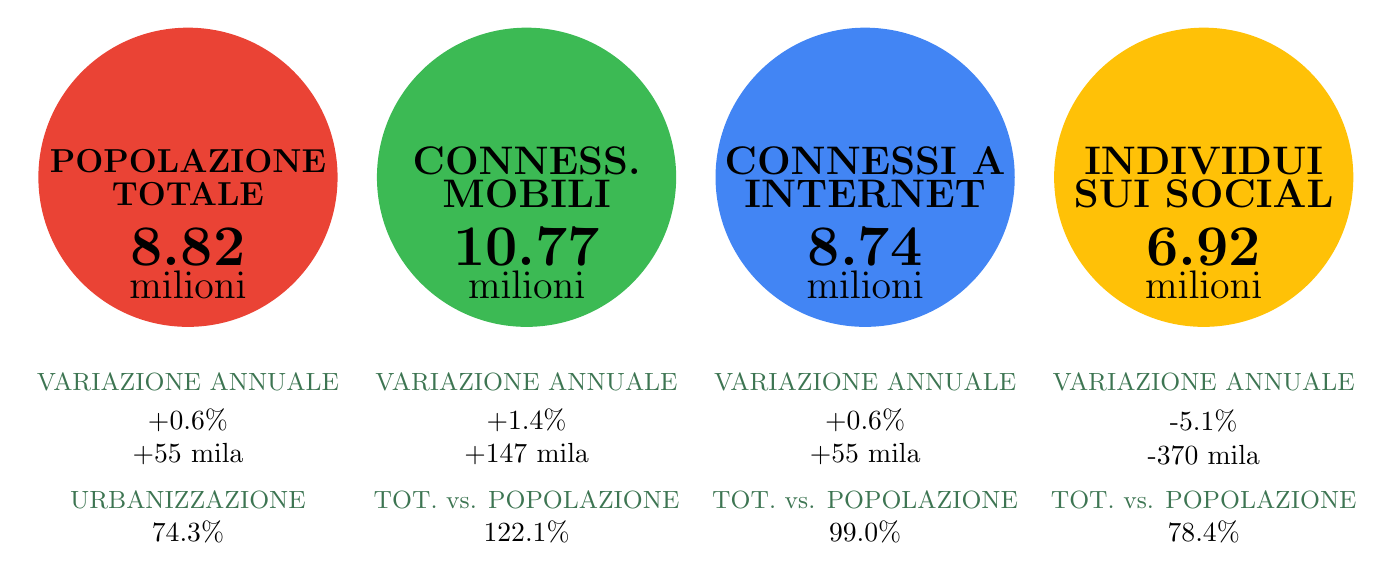
\begin{tikzpicture}
            \definecolor{textcolor}{RGB}{61,117,82}
            \definecolor{circlecolor1}{RGB}{234,67,53}
            \definecolor{circlecolor2}{RGB}{60,186,84}
            \definecolor{circlecolor3}{RGB}{66,133,244}
            \definecolor{circlecolor4}{RGB}{255,193,7}
        
            % Popolazione totale
            \fill[circlecolor1] (0,7.5) circle (1.9);
            \node[align=center] at (0,7.5) {\textbf{\large POPOLAZIONE}\\ \textbf{\large TOTALE}};
            \node[align=center] at (0,6.4) {\huge \textbf{8.82}\\ \Large milioni};
            \node[align=center, text=textcolor] at (0,4.9) {\small VARIAZIONE ANNUALE};
            \node[align=center] at (0,4.2) {+0.6\%\\ +55 mila};
            \node[align=center, text=textcolor] at (0,3.4) {\small URBANIZZAZIONE};
            \node[align=center] at (0,3) {74.3\%};
            
            % Connessioni mobili
            \fill[circlecolor2] (4.3,7.5) circle (1.9);
            \node[align=center] at (4.3,7.5) {\textbf{\Large CONNESS.}\\ \textbf{\Large MOBILI}};
            \node[align=center] at (4.3,6.4) {\huge \textbf{10.77}\\ \Large milioni};
            \node[align=center, text=textcolor] at (4.3,4.9) {\small VARIAZIONE ANNUALE};
            \node[align=center] at (4.3,4.2) {+1.4\%\\ +147 mila};
            \node[align=center, text=textcolor] at (4.3,3.4) {\small TOT. vs. POPOLAZIONE};
            \node[align=center] at (4.3,3) {122.1\%};
            
            % Connessi a internet
            \fill[circlecolor3] (8.6,7.5) circle (1.9);
            \node[align=center] at (8.6,7.5) {\textbf{\Large CONNESSI A}\\ \textbf{\Large INTERNET}};
            \node[align=center] at (8.6,6.4) {\huge \textbf{8.74}\\ \Large milioni};
            \node[align=center, text=textcolor] at (8.6,4.9) {\small VARIAZIONE ANNUALE};
            \node[align=center] at (8.6,4.2) {+0.6\%\\ +55 mila};
            \node[align=center, text=textcolor] at (8.6,3.4) {\small TOT. vs. POPOLAZIONE};
            \node[align=center] at (8.6,3) {99.0\%};
            
            % Individui sui social
            \fill[circlecolor4] (12.9,7.5) circle (1.9);
            \node[align=center] at (12.9,7.5) {\textbf{\Large INDIVIDUI}\\ \textbf{\Large SUI SOCIAL}};
            \node[align=center] at (12.9,6.4) {\huge \textbf{6.92}\\ \Large milioni};
            \node[align=center, text=textcolor] at (12.9,4.9) {\small VARIAZIONE ANNUALE};
            \node[align=center] at (12.9,4.2) {-5.1\%\\ -370 mila};
            \node[align=center, text=textcolor] at (12.9,3.4) {\small TOT. vs. POPOLAZIONE};
            \node[align=center] at (12.9,3) {78.4\%};
        \end{tikzpicture}}
    \end{center}
\end{snippet}

\end{document}